% Aufbau Kolben

    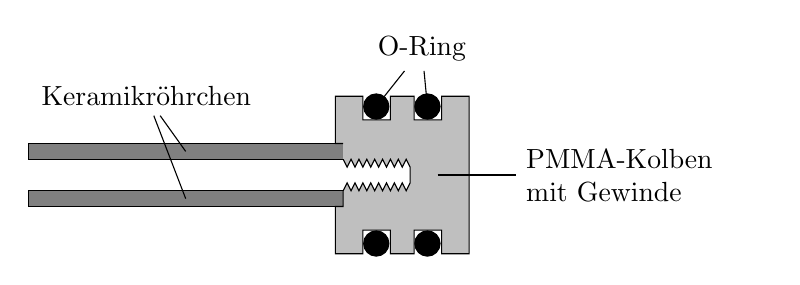
\begin{tikzpicture}
        % AlOx Rohr
        \draw[fill=gray] (0,.2) rectangle (4,.4);
        \draw[fill=gray] (0,-.2) rectangle (4,-.4);

        % Kolben
        \draw[fill=lightgray] (4.,.4) -- (3.9,.4) 
            -- (3.9,1)
            -- (4.25,1) 
            -- (4.25,.7)
            -- (4.6,.7)
            -- (4.6,1)
            -- (4.9,1)
            -- (4.9,.7)
            -- (5.25,.7)
            -- (5.25,1)
            -- (5.6,1)
            -- (5.6,-1)
            -- (5.25,-1)
            -- (5.25,-.7)
            -- (4.9,-.7)
            -- (4.9,-1)
            -- (4.6,-1)
            -- (4.6,-.7)
            -- (4.25,-.7)
            -- (4.25,-1) 
            -- (3.9,-1)
            -- (3.9,-.4)
            -- (4.,-.4)
            -- (4.,-.2)
            \foreach \x in {4.0,4.1,...,4.8} {
                -- (\x+.05,-0.1)
                -- (\x+.1,-.2)
            }
            -- (4.85,-.1)
            -- (4.85,.1)
            -- (4.8,.2)
            \foreach \x in {4.8,4.7,...,4.0}{ 
                -- (\x-.05,0.1)
                -- (\x-.1,.2)
            };

        % O-Ringe

            \draw[fill] (4.42,.87) coordinate (O1) circle(.16);
            \draw[fill] (5.07,.87) coordinate (O2) circle(.16);
        \draw[fill] (4.42,-.87) circle(.16);
        \draw[fill] (5.07,-.87) circle(.16);

        % Beschriftung

        \node (rohr) at (1.5,1) {Keramikröhrchen};
        \draw (2.,.3) -- (rohr);
        \draw (2.,-.3) -- (rohr);
        
        \node (oring) at (5.,1.6) {O-Ring};
        \draw (O1) -- (oring);
        \draw (O2) -- (oring);

        \draw (5.2,0) -- (6.2,0.0) node[right] {\parbox{3cm}{PMMA-Kolben\\ mit Gewinde}};
    \end{tikzpicture}
